%% ----------------------------------------------------------------
%% Report.tex -- MAIN FILE (the one that you compile with LaTeX)
%% ---------------------------------------------------------------- 

% Set up the document
\documentclass[a4paper, 11pt, oneside]{Thesis}  % Use the "Thesis" style, based on the ECS Thesis style by Steve Gunn
\graphicspath{Figures/}  % Location of the graphics files (set up for graphics to be in PDF format)

% Include any extra LaTeX packages required
\usepackage[square, numbers, comma, sort&compress]{natbib}  % Use the "Natbib" style for the references in the Bibliography
\usepackage{verbatim}  % Needed for the "comment" environment to make LaTeX comments
\usepackage{vector}  % Allows "\bvec{}" and "\buvec{}" for "blackboard" style bold vectors in maths
\hypersetup{urlcolor=blue, colorlinks=true}  % Colours hyperlinks in blue, but this can be distracting if there are many links.

% code
\usepackage{listings}
%\begin{lstlisting}
%Put your code here.
%\end{lstlisting}

% float H
\usepackage{float}
\renewcommand{\textfraction}{0}
\renewcommand{\topfraction}{1}
\renewcommand{\bottomfraction}{1}
\renewcommand{\floatpagefraction}{1}


\usepackage{titlesec}
 

%% ----------------------------------------------------------------
\begin{document}
\frontmatter      % Begin Roman style (i, ii, iii, iv...) page numbering

% Set up the Title Page
\title  {TFY4500 biophysics specalization project}
\authors  {\texorpdfstring
            {\href{arve@seljebu.no}{Arve Seljebu}}
            {Arve Seljebu}
            }
\addresses  {\groupname\\\deptname\\\univname}  % Do not change this here, instead these must be set in the "Thesis.cls" file, please look through it instead
\date       {\today}
\subject    {}
\keywords   {}

\maketitle
%% ----------------------------------------------------------------

\setstretch{1.3}  % It is better to have smaller font and larger line spacing than the other way round

% Define the page headers using the FancyHdr package and set up for one-sided printing
\fancyhead{}  % Clears all page headers and footers
\rhead{\thepage}  % Sets the right side header to show the page number
\lhead{}  % Clears the left side page header

\pagestyle{fancy}  % Finally, use the "fancy" page style to implement the FancyHdr headers

%% ----------------------------------------------------------------
\chapter{Summary}

In the search for curing cancer researchers have had a clear focus on understanding tumor cells. Though still outnumbered by the number of published articles on tumor cells, studies focusing on tumor cell environment is getting traction. Some studies have shown that the tumor environment, also known as the tumor stroma, may have significant impact on development of a tumor. It's suspected that connective and supporting tissue in the tumor stroma have a significant role in the metastasis, the state when tumor cells spreads to new parts of the body.

In fact research suggest that there is a correlation between structure of collagen tissue and survival of the patient. This can be used in diagnosis, but also suggest that there might be possibilities to avoid cancer cells spreading by altering the tumor stroma. This report will focus on the diagnosis part, in specific on collagen tissue from breast cancer.

In example, one property of tissue structure is alignment and curliness of collagen fibers. An earlier study at NTNU have measured curliness and alignment properties in a manual qualitative manner on a data set of 37 samples. The purpose of this report is documenting project work that has been done on automating the process such that a larger data set can be obtained and studied. To be specific, the project have explored possibilities for obtaining large number of high quality images of breast tissue samples with automated nonlinear microscope scanning. The project have also created some quantitative data from the images.

The goal for this report is informing about the process and the results. The details are:
\begin{itemize}
\item Find good parameters for obtaining high quality images
\item Find an effective way to scan whole glass slides of 135 samples with little human intervention
\item Store the images in a structured manner so that 
    \begin{itemize}
    \item Correlation to patient data is possible
    \item Quantitative data can be subtracted
    \end{itemize}
\item Try some algorithms for creating quantitative data
\end{itemize}

\textbf{The results are:}
\begin{itemize}
\item  Nonlinear scanning microscope with femto-second laser and non-descanned sensors give images with visible fiber structures. Photonmultiplier tubes (PMT) are subject to more noise than hybrid detectors (HyD), but PMT are more reliable when sample contain areas of very high intensity.
\item Having a way to adjust plane of sample making it horizontal is crucial for scanning an area of $\approx 3$ cm$^2$ without loosing focus. Microscope software should also have a way to define plane of focus before starting the scan, as auto focusing all coordinates is not a viable option due to time constraints, adding 7+ hours to the scan. Using auto focus at regular intervals are neither an option, as it may hit a coordinate with no signal which results in selecting focus at random. It is hard to find a reliable process to detect if little signal is due to focus problems after the scan have been done and it's also cumbersome to rescan selective parts of the glass slide. Tweaking settings of microscope, making xyz-coordinates easily available and storing spatial positions in memory, makes aligning of the sample before scan more effective.
\item Selecting and grouping specific part of the glass slide already at scanning is preferred, as diving the scan images into groups representing one sample is non-trivial for a data set containing 3-4000 images. In contrast, grouping samples when scanning makes image processing and keeping record of spatial placement to specific tissue samples a trivial task.
\item Quantifying fiber direction with Fourier transform gives a feature that possibly can be used in classification to separate anisotropic samples from samples having fibers in a few specific directions. Using gradients for creating features have not been successful.
\end{itemize} % Summary

\setstretch{1.3}  % Reset the line-spacing to 1.3 for body text (if it has changed)
\pagestyle{fancy}  %The page style headers have been "empty" all this time, now use the "fancy" headers as defined before to bring them back


%% ----------------------------------------------------------------
\lhead{\emph{Contents}}  % Set the left side page header to "Contents"
\tableofcontents  % Write out the Table of Contents


%% ----------------------------------------------------------------
\mainmatter	  % Begin normal, numeric (1,2,3...) page numbering
\pagestyle{fancy}  % Return the page headers back to the "fancy" style
\lhead{} % empty left side header

% Include the chapters of the thesis, as separate files
% Just uncomment the lines as you write the chapters

\chapter{Introduction}

Over three million published articles on pubmed with keyword \textit{cancer} shows the huge amount of research effort for understanding, diagnosing and treating cancer diseases. The research focus is mainly on tumor cells, but a segment of interest which is increasing is research on tumor stroma as seen in figure \ref{fig:pubmed}. Tumor stroma is basically the environment of cells that is suppressing or supporting the function of the tumor cells. It is suggested that under the development of a tumor, the stroma is changing from being suppressive to supportive of the tumor cells.

\begin{figure}[h]
\centering
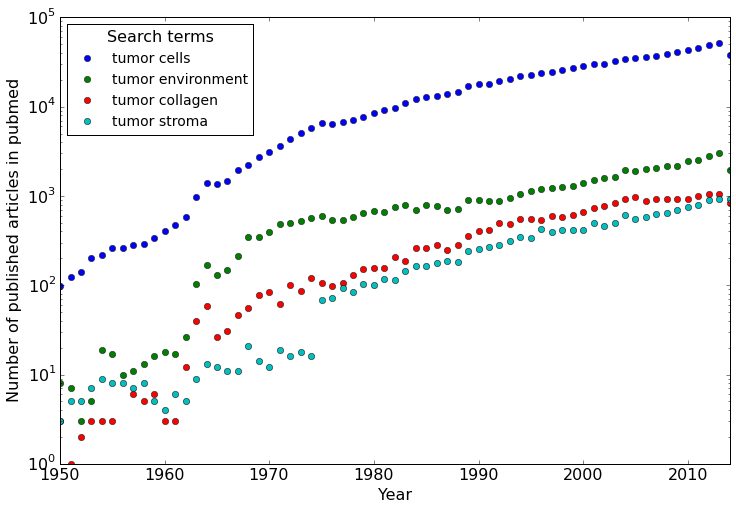
\includegraphics[width=10cm]{pubmed_tumor}
\caption{Amount of published articles by year on different search terms. The search term \textit{tumor cells} outnumber the others by two orders of magnitude. Note the logarithmic scale on y-axis.}
\label{fig:pubmed}
\end{figure}

In particular, collagen fiber is known to be altered in the surroundings of tumor cells under the development towards metastasis. One bio-marker for collagen fibers, is their alignment at the vincinity of the tumor, which may predict if a tumor is malignant. The fiber alignment can be used as a diagnosis tool for malignant tumor, and an article written at NTNU have studied collagen fiber alignment in a manual qualitative manner \cite{anna}.

St. Olav hospital have taken breast tissue samples from 900 pasients. In total three samples per patient, one sample inside, one sample at the boundary and one sample outside the tumor. The samples is laid in a matrix on a glass slide, each glass slide having about 130 samples. As microscope scanning and analysis of such a large data set is not straightforward, this project have explored possibilities for automating the process.

To be specific, the goals of the project were:
\begin{itemize}
\item  Find good parameters for obtaining high quality images
\item Find an effective way to scan whole glass slides of 135 samples with little human intervention
\item Store the images in a structured manner so that 
    \begin{itemize}
    \item Correlation to patient data is possible
    \item Quantitative data can be subtracted
    \end{itemize}
\item Try some algorithms for creating quantitative data
\end{itemize} % Introduction

\chapter{Theory}

%
% IMAGE PROCESSING
%
\section{Image processing}
\subsection{Representation}
All images in this report are two dimensional arrays of integer values. The image is denoted $f(x,y)$, where $f(0,0)$ is the intensity value of the top left pixel. Positive direction for x and y-axis is respectively right and down as seen in figure \ref{fig:equalized} (a). Pixel axis will be omitted unless useful for description of image.

\begin{figure}
\centering
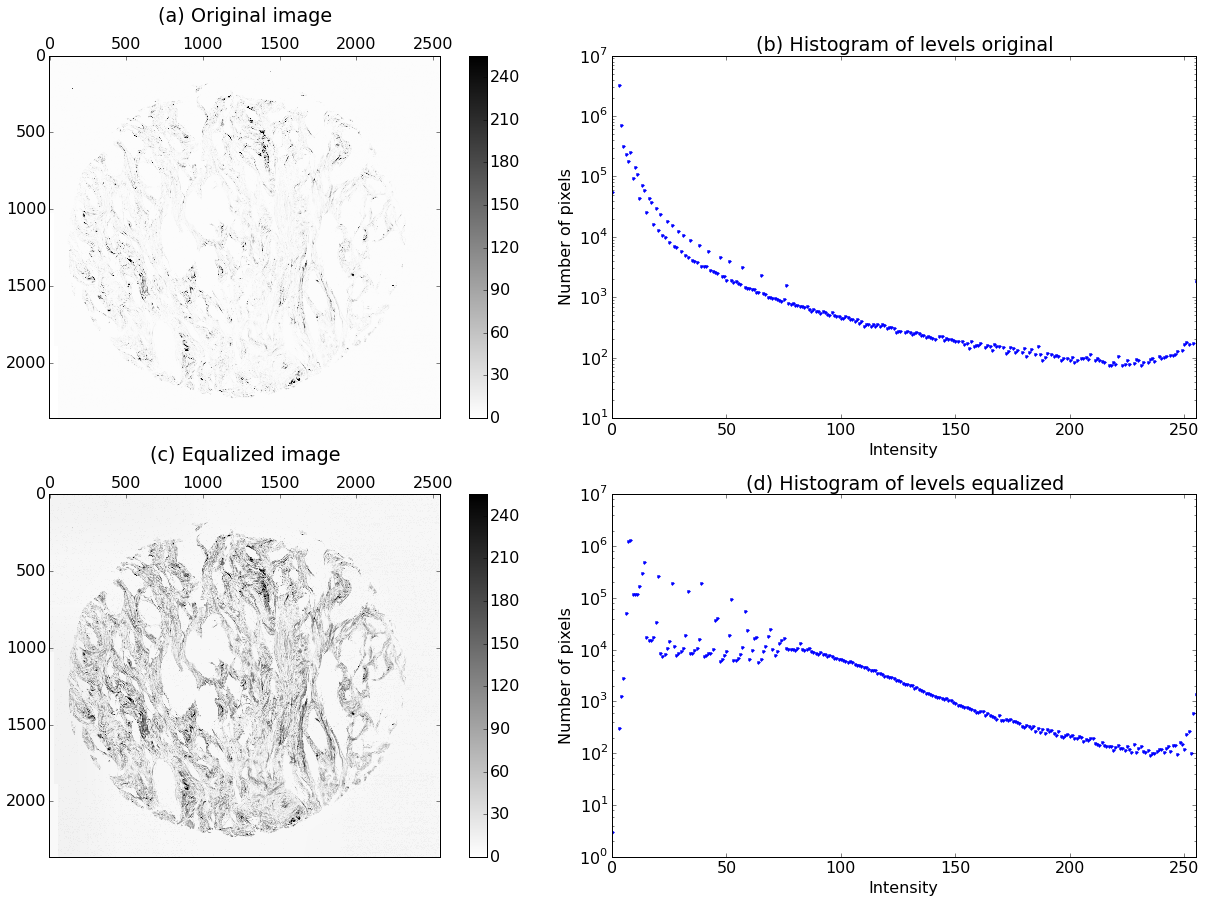
\includegraphics[width=14cm]{equalized}
\caption{(a) Original image from microscope. (b) Histrogram of intensity values in image (a). (c) Adaptive histogram equalization of image (a). (d) Histogram of intensity values in image (c). Note that the scale of the y-axis in the histograms are logarithmic. }
\label{fig:equalized}
\end{figure}

An image intensity value of zero equals no signal and representation is dependt on colormap chosen. As microscope images in this report tend to have a lot of near zero pixel values, an inverted colormap is used for better visibility. In other words zero are represented as white, in contrast to black that one might assume. As long as possible, the same colormap is used on same type of images. It is suggested that the reader note the colorbar beside the image which indicate correspondence between numerical value and color.

\subsection{Contrast enhancement}
Images where structures are more important than the numerical values, \textit{histogram equalization} is used to enhance contrast. Histogram equalization tries to make each intesity likely probable, which often result to a higher contrast and therefor better visibility. An example is shown in figure \ref{fig:equalized}, where (a) is the original image and (c) is the equalized image. The algorithm used to equalize figure \ref{fig:equalized} (c) is called \textit{adaptive histogram equalization} and are found in the python library scikit-image. As this are just for visibility in the report, it’s suggested to read scikit-image documentation or source code if more detail is needed. Figure caption will always note if images has been processed with any kind of contrast enhancement method.

%
% SCANNING MICROSCOPE
%
\section{Scanning microscope}
The microscope in use is a scanning microscope. It’s called scanning due to the moving mirror which directs the laser to different spatial coordinates on the sample. The laser will move in a raster pattern and a sensor detect light in samples. Each sample represent one pixel and computer software assign the sensed values to a digital image. By scanning speed, we mean the count of lines scanned per second. In example a scanning speed of 600 Hz will use 853 milliseconds to scan a whole image of 512x512 pixels.

As it’s possible to control the amplitude of the mirror oscillation, choosing a smaller amplitude of the oscillation will effectively zoom. This gives the user of a scanning microscope control over spatial resolution without changing objective. Though the zooming is not without limitation, as too high oscillation frequency could damage the mirror. In example, a high mirror oscillation frequency would limit the possible amplitude which effectively limits how low zoom one can use.

Even if it's possible in software to select resolution below the theoretical resolution defined by the Rayleigh criterion, we are still limited by the diffraction limit. Resolution is therefor given by

\begin{equation}
d = 0.61 \cdot \frac{\lambda}{NA}
\end{equation}

where $\lambda$ is wavelenght of light and $NA$ is numerical aperture of objective.

%
% NONLINEAR LIGHT INTERACTION
%
\section{Nonlinear light interaction}
%Signal, noise, sampling, instrumentation
Second harmonic generation (SHG) is a interaction between photons and material which generate light of twice the frequency as the incomming light. The generation is due to the material's nonlinear susceptibility, which can be explained by the polarized density

\begin{equation}
\vec{P} = \chi_1 \vec{E} + \chi_2 \vec{E} \cdot \vec{E} + \chi_3\vec{E} \cdot \vec{E} \cdot \vec{E} + ...
\end{equation}

When a material have $\chi_2 \neq 0$, two photons may interact with the material to create a polarized field. The polarized field then again generates an $\vec{E}$-field with twice the frequency as the incoming light (two photons interact with the material, creating a single photon with twice the energy). The interaction only happens upon a high intensity beam where two photons are at the same place at the same time. Practically this is achieved by using a pulsed laser and focusing the beam with an objective, as a steady beam of this intensity magnitude would damage the sample. Also since the probability for interaction is proportional to intensity squared, one get the convenient benefit of essentially no SHG outside the focal point.

$\chi_2$ is also dependent on wavelength of incoming light and properties of the material, which results in material needs to be non-centrocymetric. This happens to be the case for collagen fibers as some of few biological materials, making it simple to take images of the collagen fibers only with little sample preparation.

The pulsed laser is normally scanned over the sample, generating SHG-signal and detected by sensors. As compared to a confocal microscope, descanning of the light is not necessary to take away background signal. 

%
% FOURIER TRANSFORM
%
\section{Forier transform}
A common way to view data is in it's frequency domain. To achieve this, one does a Fourier transform defined by

\begin{equation}
F\{f(t)\} = \int \limits_{-\infty}^{\infty} f(t) e^{-i2\pi \mu t} dt.
\end{equation}

The transform has the property that it "picks out" amplitude and phase of oscillating signals in $f(t)$. This is based on the Fourier series which states that any periodic function can be represented by a sum of finite or infinite set of sines and cosines.

As we are working with images in the discrete domain, one defines $f(t)$ to be a sampled function using the Dirac delta function and gets the discrete Fourier transform

\begin{equation}
F(u) = \sum \limits_{x=0}^{M-1} f(x)e^{-i2 \pi ux/M}.
\end{equation}

Where $u$ and $x$ are discrete values for frequency and position, and M is number of samples in the function $f(x)$. Adding a dimension yields the 2D discrete Fourier transform given by

\begin{equation}
F(u,v) = \sum \limits_{x=0}^{M-1} \sum \limits_{y=0}^{N-1} f(x,y) e^{-i2 \pi \left( \frac{ux}{M} + \frac{vy}{N} \right)}.
\end{equation}

Here $u$ and $v$ are frequencies for accordingly $x$ and $y$ dimensions in the real image $f(x,y)$. $M$ and $N$ are the size of the image. The transform yields an image with same dimensions as the real image, where $F(u,v)$ gives amplitude and phase of given frequencies $u$ and $v$. All Fourier images in this report are logarithms of power spectrum which are shifted. The power spectrum of the Fourier transform is given by

\begin{equation}
|F(u,v)| = \sqrt{F(u,v) \cdot \overline{F(u,v)}},
\end{equation}

where $\overline{F(u,v)}$ is the complex conjugate of $F(u,v)$. Values below 1 are set to 1, to avoid division by zero and $-\infty$ values. Because the domain of values may range $10^6$ in the power spectrum, logarithmic scaling is done. In example the Fourier spectrum to figure \ref{fig:ft_demo} (a), have a maximum value of $8 \cdot 10^6$. Shifting means that $u=0$ and $v=0$ are set to the center of the image, as it's easier to grasp what frequencies are involved and direction of features in the image.

\begin{figure}[h]
\centering
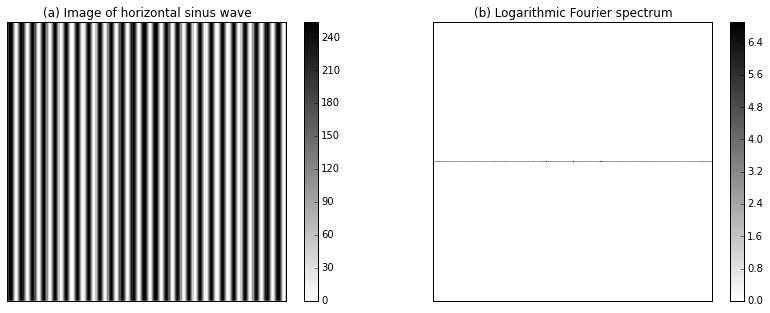
\includegraphics[width=11cm]{ft_demo.png}
\caption{(a) An 8 bit grayscale image with sine wave running in x-direction. (b) The logmarithmic scaled power spectrum of the Fourier transform. The Fourier transform has been shifted for better visibility, as we have no repeating signal in y-direction and the line actually lays on the border of the image ($v$ = 0).}
\label{fig:ft_demo}
\end{figure}

As mentioned, the transform picks out amplitude, phase and frequency, which are properties we can exploit to find orientation of fibers. Figure \ref{fig:ft_demo} shows this concept.


%
% CLASSIFICATION
%
%\section{Classification}
%Magnus: Mulig jeg må droppe dette, ser ikke ut som jeg kommer i mål.

%As the goal for automated analysis is making decisions, quantitative data is used to separate samples into classes. In best case scenario a few quantitative measurement clearly discriminates the samples. Figure \ref{fig:iris} of the classical iris data-set from R.A. Fisher illustrates this concept.

%\begin{figure}
%\centering
%\includegraphics[width=5cm]{iris.png}
%\caption{Three different species of iris flowers, discriminated by their pedal and sepal width. Data from http://archive.ics.uci.edu/ml/datasets/Iris. TODO fix ref}
%\label{fig:iris}
%\end{figure}

%As the figure show, grouping classes based on their quantitative measurements is a simple concept, but it gets complicated when the data span more dimensions that the human mind can easily visualize. To improve our ability to find good classifiers one technique is to use machine learning. The concept is the same, but one lets a computer find which measurements gives good separation of classes. This is done by iteratively computing distance to the mean position of predefined classes. Mean distance is defined as

%\begin{equation}
%\mathbf m_j = \frac{1}{N_j} \sum\limits_{\mathbf x \in \omega_j} \mathbf x_j
%\end{equation}

%where $N_j$ is the number of vectors in class $\omega_j$.


%A simple but effective implementation of this is clustering measurements 
%find quantitative measures that disciminates the samples to classes % Background Theory 

\chapter{Method}

%
% SAMPLES
%
\section{Sample slide}

\begin{figure}[h]
\centering
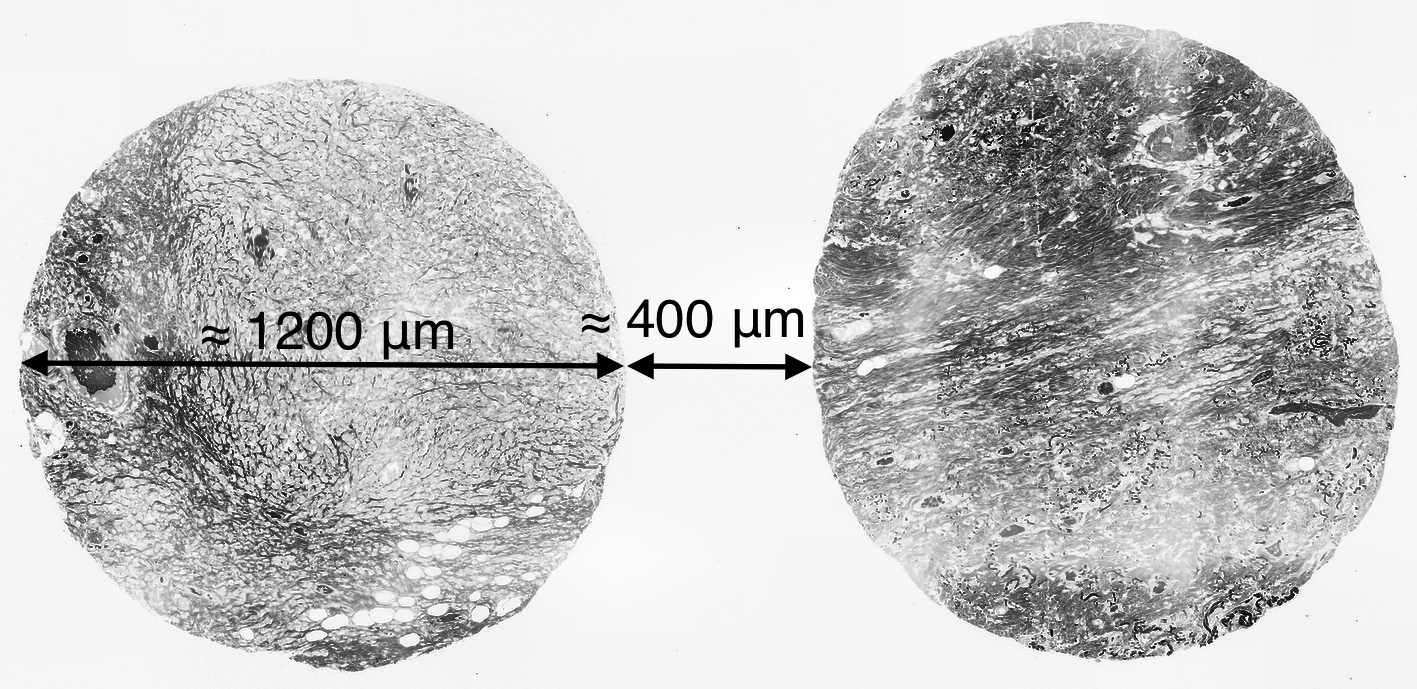
\includegraphics[width=8cm]{spots}
\caption{Two spots side by side with approximate sizes. The left spot have more circular shape than the right one. }
\label{fig:spots}
\end{figure}

Each glass slide contains 9x15 sample spots of breast tissue with diameter $\approx$ 1200 $\mu$m, \\ $\approx 0.4$ mm spacing between and 5 $\mu$m thickness. An illustration taken with fluorescence microscopy of a stained sample is shown in figure \ref{fig:spots}. All other images in this report is unstained samples. Some of the sample spots seem transparent to human eye and give little or no SHG-signal. It has not been confirmed if this is due to failure in sample preparation or if the tissue is transparent.

\begin{figure}[h]
\centering
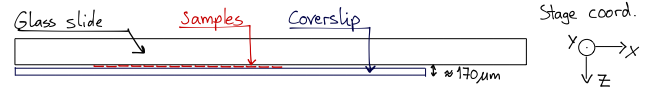
\includegraphics[width=10cm]{tilt}
\caption{Illustration of glass slide with coverslip mounted too far to the left, leaving no room for resting the glass slide on the microscope stage.}
\label{fig:tilt}
\end{figure}

When glass slide is lying on the microscope stage, sample plane is measured to have tilt by $\approx$ 170  $\mu$m in x-direction due to misaligned coverslip (illustrated in figure \ref{fig:tilt}) and $\approx 70 \mu$m in y-direction (unknown cause, might be microscope sample holder).


%
% INSTRUMENTATION
%
\section{Instrumentation}

\subsection{Microscope}
The project used a Leica SP8 microscope with Leica LAS AF software version 3.3.0.10134. Objectives in microscope are shown in table \ref{tab:objectives}. Laser of microscope is a Chameleon Vision-S from Coherent with 80Mhz pulsing frequency and $\approx$ 75 picoseconds pulse width rated to 2.5 Watt. In all images 890 nanometer was used and output power was shown in the software to be $\approx$ 1950 mW.

\begin{center}
 \begin{tabular}{|c c c|} 
 \hline
 Mag/NA & Immersion & Name \\ [0.5ex]
 \hline\hline
 20x/0.75 & None & HC PL APO \\ 
 \hline
 25x/0.95 & Water & HCX IRAPO \\ 
 \hline
 63x/1.20 & Water & HC PL APO \\
 \hline
 63x/1.40 & Oil & HC PL APO \\
 \hline
\end{tabular}
\label{tab:objectives}
\end{center}



%
% SEMI AUTOMATIC IMAGE COLLECTION
%
\section{Semi-automatic image collection}
Two types of semi-automatic scan jobs were used in the Leica LAS AF software; \textit{tile} and \textit{matric} scan. Before scanning, sample was aligned by using the controlling touch screen seen in figure \ref{fig:touch}.

\begin{figure}[h]
\centering
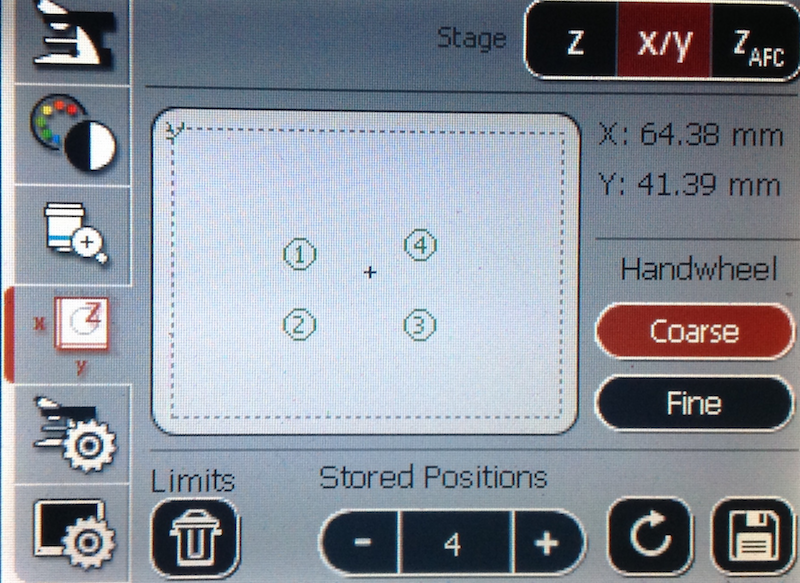
\includegraphics[width=0.66\textwidth]{touch}
\caption{Touch screen with four stored positions.}
\label{fig:touch}
\end{figure}


\subsection{Tile scan}
Tile scan is a feature in the standard view of Leica LAS AF. In tile scan one defines two points which makes a rectangle. Several scan jobs can be made, but is no way to control different jobs to different tiles, which means any job defined will run on all tiles. Auto focusing can be either all tiles or at regular intervals.

\begin{figure}[h]
\centering
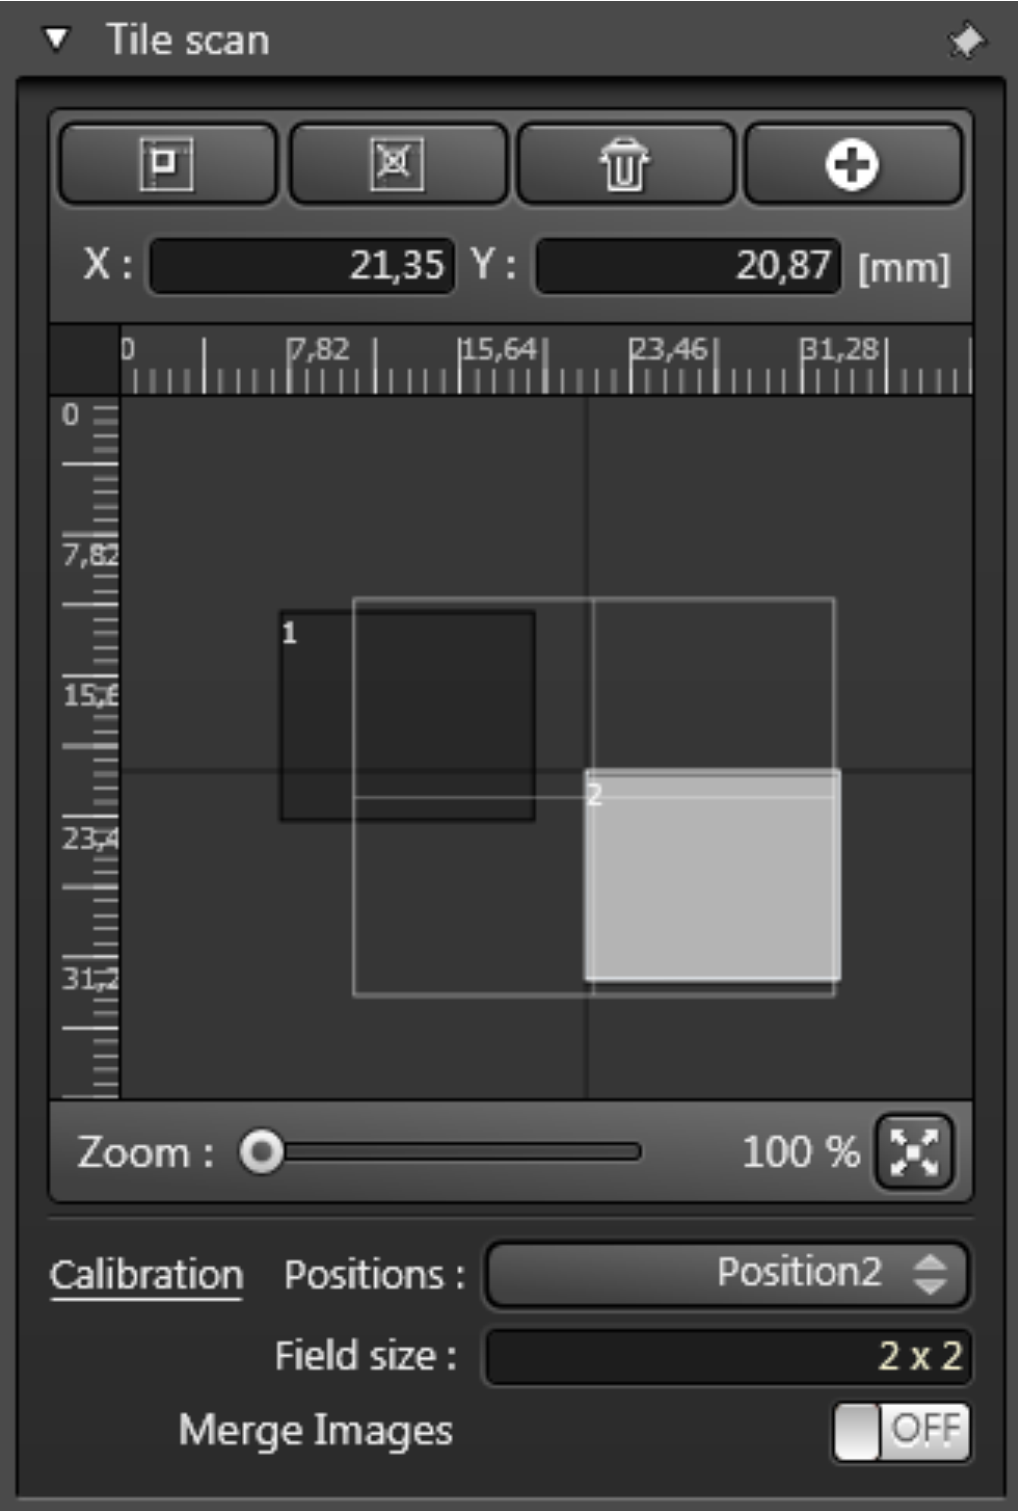
\includegraphics[width=0.33\textwidth]{tilescan}
\caption{Leica LAS AF tile scan feature. Two points define an area of tile images. Images are stored in sequence with numbers and software may also merge images.}
\label{fig:tilescan}
\end{figure}


\subsection{Matrix scan}
Matrix scan is a feature that splits a scan into so called \textit{wells} and \textit{scan fields}. This is illustrated in figure \ref{fig:wells} which have 3x2 wells with 5x5 scan fields. Each well will represent a sample spot.

\begin{figure}[h]
\centering
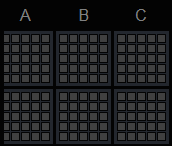
\includegraphics[width=4cm]{wells}
\caption{3x2 wells, each well containing 5x5 scan fields.}
\label{fig:wells}
\end{figure}

The matrix scan allows for individual adjusting placement of wells and focus of scan fields, making it very flexible. After the matrix scan, images are stitched with ImageJ to form one image per well.


%
% ALGORITHMS
%
\section{Algorithms}
Two types of processing have been tried out for quantifying the images, namely gradient and Fourier transform. The product of the algorithms is a histogram of angles.


\subsection{Histogram of oriented gradients}
As the name implies, this algorithm calculates gradient of an image and then use the direction of that gradient to create a histogram of angles. The algorithm is straight forward:

\begin{lstlisting}
calculate gradient
calculate angle of gradient
add every angle to histogram weighted by the gradient magnitude
\end{lstlisting}


\subsection{Frequency domain}
Two types of strategies was tried out in the frequency domain. The first technique described in psuedo code:

\begin{lstlisting}
divide image into sub images of 100x100 pixels
for every sub image:
    if mean intensity < 1: do next sub image
    do Fourier spectrum
    threshold Fourier spectrum
    do line fit
    find angle of fitted line
    add angle to histogram
\end{lstlisting}

An example of the line fitting is illustrated in figure \ref{fig:ft_good}.

\begin{figure}[h]
\centering
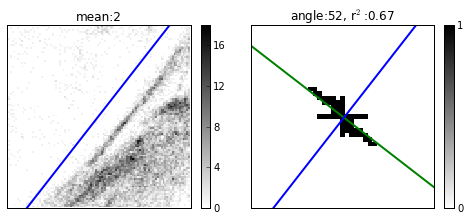
\includegraphics[width=0.5\textwidth]{ft_line_good}
\caption{Example of line fitting in Fourier spectrum. Fourier spectrum have been zoomed, omitting a border of 30 empty pixels.}
\label{fig:ft_good}
\end{figure}

The second technique is similar:

\begin{lstlisting}
do Fourier spectrum
threshold Fourier spectrum
for every pixel in tresholded Fourier spectrum:
    find angle
    add angle to histogram
\end{lstlisting}
 % Experimental Setup, software algorithms

\chapter{Result}
%
% SETTINGS
%
\section{Scan settings}
Figure \ref{fig:obj_comparison} show a comparison of a 20x dry objective to a 63x water objective. Note that (a) have stronger signal.

\begin{figure}[h]
\centering
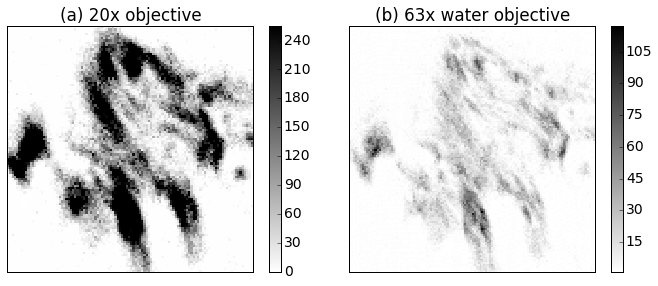
\includegraphics[width=\textwidth]{objectives}
\caption{Comparison of 20x dry objective to 63x water objective. Note that picture (a) have several pixels with maximum value (255). Settings for image (a) are PMT-gain of 700 Volt and scanning speed 400 Hz. Settings for image (b) are PMT-gain of 650 Volt and scanning speed 200 Hz.}
\label{fig:obj_comparison}
\end{figure}

Power equal 10\%, gain 60\% and offset 50\% for laser at 890 nm was found to create images taking use of whole 8 bit intensity range when PMT detector had gain of $\approx$ 600 Volt, but not the whole range of the HyD detector. Also some bright spots will make HyD detector shut down, giving large areas with zero value seen in figure \ref{fig:hyd}.

\begin{figure}
\centering
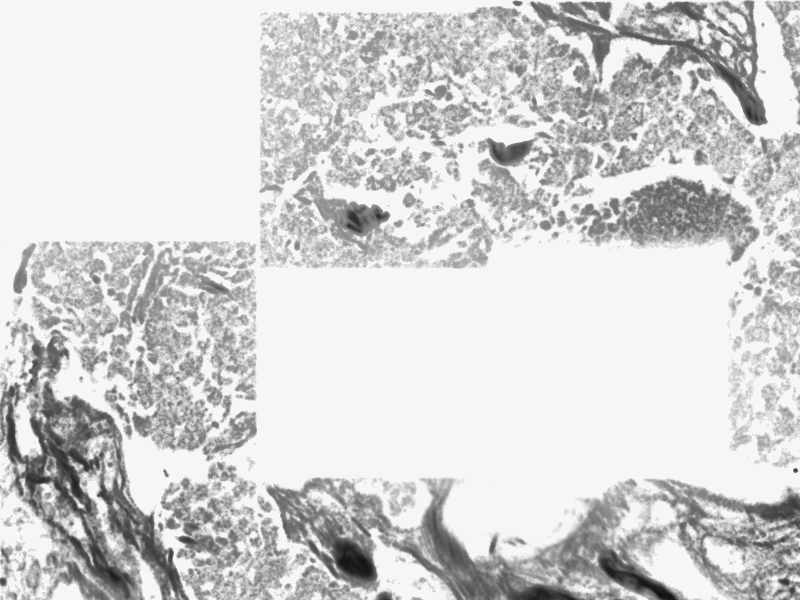
\includegraphics[width=0.5\textwidth]{hyd}
\caption{HyD detector have been shut off due to too strong signal. Image contrast is enhanced to improve visibility.}
\label{fig:hyd}
\end{figure}
 
Table \ref{tab:obj_time} show the minimum time for scanning an area of $\approx$ 1.2x1.2 mm$^2$ with pixel resolution below 200 nm. All times are given with scanning speed 600 Hz, which is the highest possible mirror oscillation frequency when using zoom factor 0.75 (minimum zoom factor possible).

\begin{table}[h]
\centering
\begin{tabular}{c c c c c c}
\hline
Objective & Zoom & Image size & Pixels & Number of images & Total time\\
\hline
20x & 0.97 & 600 $\mu$m & 4192 & 2x2 = 4 & 28 s \\
25x & 1.09 & 400 $\mu$m & 2048 & 3x3 = 9 & 31 s \\
63x & 0.92 & 200 $\mu$m & 1024 & 6x6 = 36 & 61 s \\
\hline
\end{tabular}
\caption{}
\label{tab:obj_time}
\end{table}


%
% TILESCAN VS WELLS
%
\section{Structured scan}
Figure \ref{fig:res_tilescan} show a merged tilescan. Note that several spots are uneven and that spots on left side are clipped of. Another defect is lower intensities at merging boarder, which is not easy to spot in the zoomed out figure \ref{fig:res_tilescan}, but is clearly seen in figure \ref{fig:spots}.

\begin{figure}[h]
\centering

\includegraphics[width=\textwidth]{result_tilescan}
\caption{Fluorescence tile scan with autofocus at regular intervals. Image is merged with Leica LAS AF.}
\label{fig:res_tilescan}
\end{figure}

Figure \ref{fig:single} shows an image taken with matrix scan. The image was merged from 5x5 scan fields, saving 11 images per well by omitting some of the sample.

\begin{figure}[h]
\centering
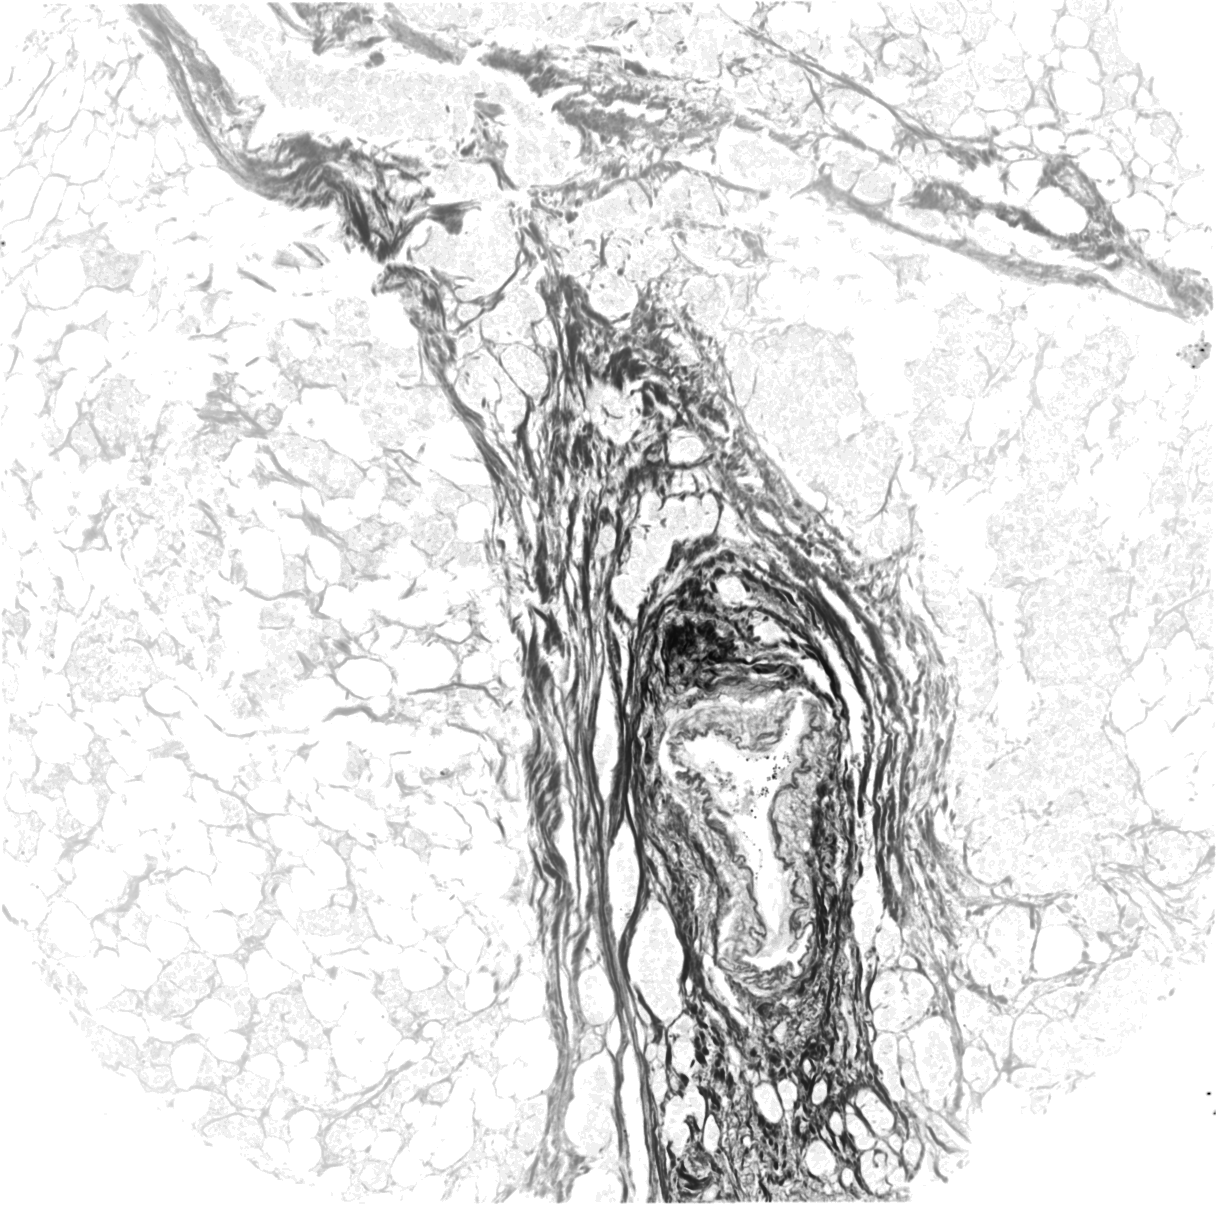
\includegraphics[width=0.33\textwidth]{single}
\caption{SHG image taken with matrix scan. Image have been merged with ImageJ and contrast enhanced with scikit-image. Area of image is 1136x1136 $\mu$m$^2$.}
\label{fig:single}
\end{figure}


%
% QUANTITATIVE
%
\section{Quantitative data}
Three samples have been picked out to illustrate the quantitative results. One image with fibers aligned in mostly one direction, one image with fibers in several directions and one image that seem anisotropic to human eye.

% HOG
% 
\subsection{Histogram of oriented gradients}
Figure \ref{fig:hist_grad_one}, \ref{fig:hist_grad_several} and \ref{fig:hist_grad_anisotropic} show histogram of angles calculated by the histogram of angles algorithm. Histogram of angles to all images have very strong response for angles 0, 45, 90 and 135, showing the weakness of calculating gradient on two dimensional data.

\begin{figure}[H]
\centering
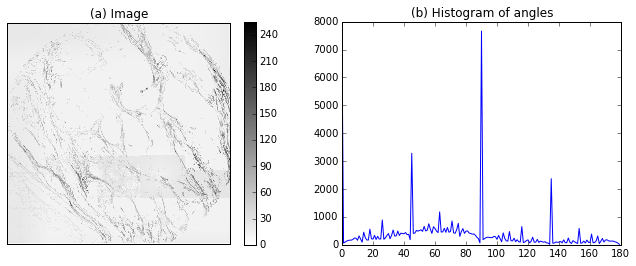
\includegraphics[width=0.8\textwidth]{hist_grad_one}
\caption{(a) Image of fibers in mostly one direction. (b) Histogram of angles calculated from gradient to image (a). A response between 40 and 90 is seen if one compare this histogram with figure \ref{fig:hist_grad_several} and \ref{fig:hist_grad_anisotropic}.}
\label{fig:hist_grad_one}
\end{figure}

\begin{figure}[H]
\centering
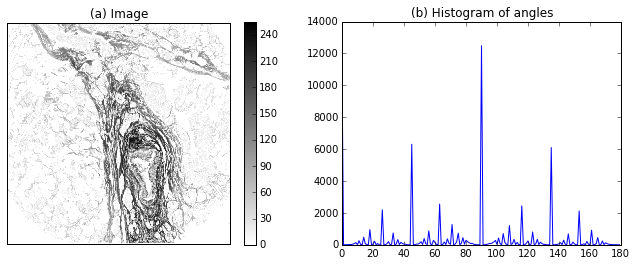
\includegraphics[width=0.8\textwidth]{hist_grad_several}
\caption{(a) Image with fibers in several directions. (b) Histogram of angles calculated from gradient to image (a). Histogram doesn't seem to contain any information about the direction of fibers in the image.}
\label{fig:hist_grad_several}
\end{figure}

\begin{figure}[H]
\centering
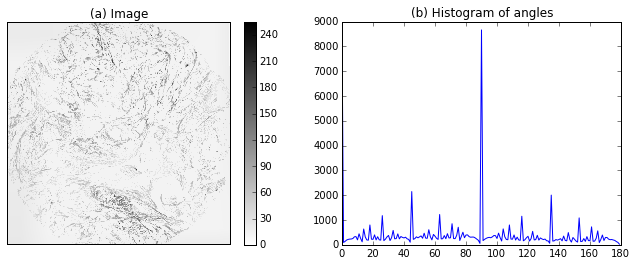
\includegraphics[width=0.8\textwidth]{hist_grad_anisotropic}
\caption{(a) Image which seems to be anisotropic to human eye. (b) Histogram of angles calculated from gradient of image (a). Histogram is very similar to figure \ref{fig:hist_grad_several} (b).}
\label{fig:hist_grad_anisotropic}
\end{figure}


% LINE
%
\subsection{Fourier transform}
\subsubsection{Line fit}
Figure \ref{fig:hist_line_one}, \ref{fig:hist_line_several} and \ref{fig:hist_line_anisotropic} show histogram of angles calculated by fitting a line in the Fourier spectrum. All images have similar response with high count of angles around 0 and 90 degrees.

\begin{figure}[h]
\centering
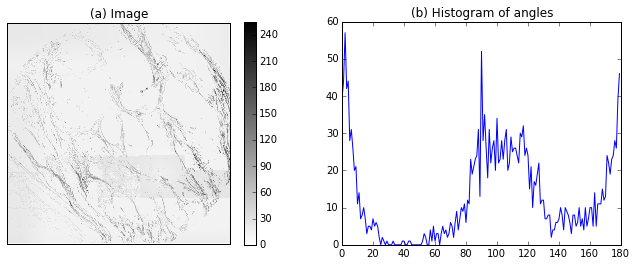
\includegraphics[width=0.8\textwidth]{hist_line_one}
\caption{(a) Image of fibers in mostly one direction. (b) Histogram of angles calculated by using line fit in Fourier spectrum.}
\label{fig:hist_line_one}
\end{figure}

\begin{figure}[h]
\centering
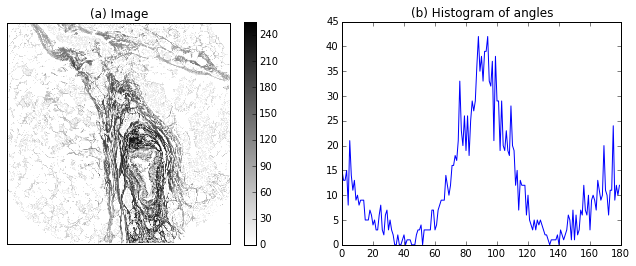
\includegraphics[width=0.8\textwidth]{hist_line_several}
\caption{(a) Image with fibers in several directions. (b) Histogram of angles calculated by using line fit in Fourier spectrum.}
\label{fig:hist_line_several}
\end{figure}

\begin{figure}[h]
\centering
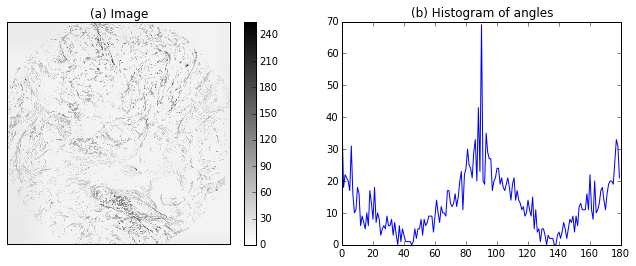
\includegraphics[width=0.8\textwidth]{hist_line_anisotropic}
\caption{(a) Image which seems to be anisotropic to human eye. (b) Histogram of angles calculated by using line fit in Fourier spectrum.}
\label{fig:hist_line_anisotropic}
\end{figure}


As figures \ref{fig:hist_line_one}, \ref{fig:hist_line_several} and \ref{fig:hist_line_anisotropic} show similar response, lines with a bad fit where discarded making figure \ref{fig:hist_line_one3}, \ref{fig:hist_line_several3} and \ref{fig:hist_line_anisotropic3}. Lines with correlation coefficient r$^2$ below 0.3 are discarded.


\begin{figure}[h]
\centering
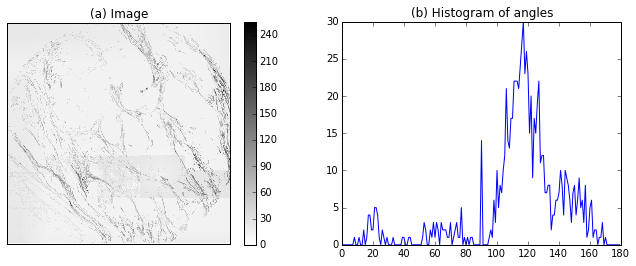
\includegraphics[width=0.8\textwidth]{hist_line_one3}
\caption{(a) Image of fibers in mostly one direction. (b) Histogram of angles calculated by using line fit in Fourier spectrum. Lines with r$^2$ < 0.3 are discarded. A clear response at about 120 degree is shown.}
\label{fig:hist_line_one3}
\end{figure}

\begin{figure}[h]
\centering
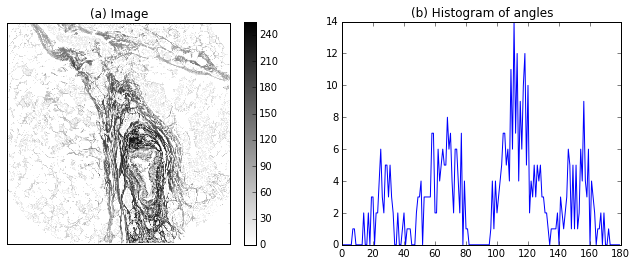
\includegraphics[width=0.8\textwidth]{hist_line_several3}
\caption{(a) Image with fibers in several directions. (b) Histogram of angles calculated by using line fit in Fourier spectrum. Lines with r$^2$ < 0.3 are discarded. Four clusters of angles are shown, $\approx$ 100-120 degree being the strongest response.}
\label{fig:hist_line_several3}
\end{figure}

\begin{figure}[h]
\centering
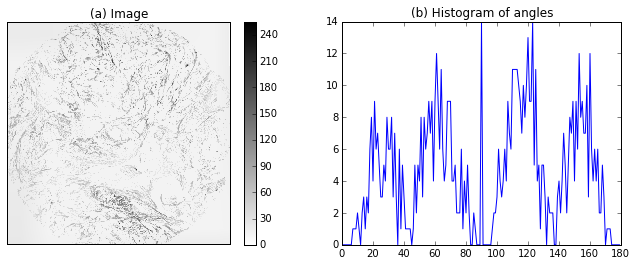
\includegraphics[width=0.8\textwidth]{hist_line_anisotropic3}
\caption{(a) Image which seems to be anisotropic to human eye. (b) Histogram of angles calculated by using line fit in Fourier spectrum. Lines with r$^2$ < 0.3 are discarded. Four roughly equal cluster of angles are shown.}
\label{fig:hist_line_anisotropic3}
\end{figure}


% SUM
%
\subsubsection{Sum of angles}
Figure \ref{fig:hist_sum_one}, \ref{fig:hist_sum_several} and \ref{fig:hist_sum_anisotropic} show histogram of angles calculated by summing up angles of top intensity pixels in Fourier spectrum.

\begin{figure}[h]
\centering
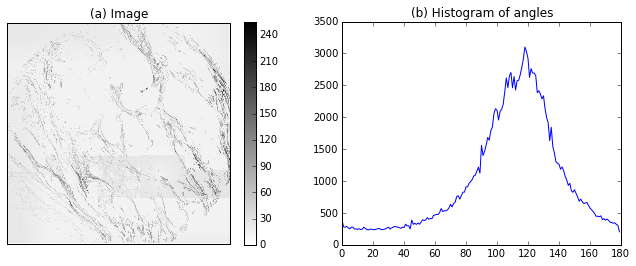
\includegraphics[width=0.8\textwidth]{hist_sum_one}
\caption{(a) Image of fibers in mostly one direction. (b) Histogram of angles calculated by summing up the angle of top intensity pixels in Fourier spectrum. Histogram have a peak at $\approx$ 125 degree with $\approx$ 40 degrees width.}
\label{fig:hist_sum_one}
\end{figure}

\begin{figure}[h]
\centering
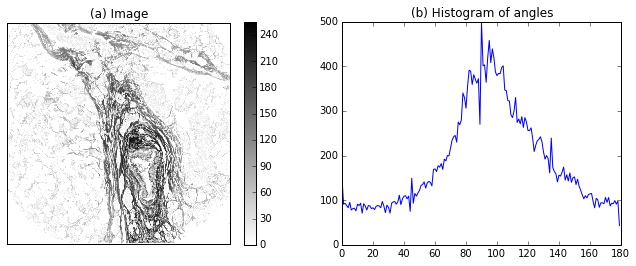
\includegraphics[width=0.8\textwidth]{hist_sum_several}
\caption{(a) Image with fibers in several directions. (b) Histogram of angles calculated by summing up the angle of top intensity pixels in Fourier spectrum.
Histogram have a peak at $\approx$ 95 degree with $\approx$ 50 degrees width.}
\label{fig:hist_sum_several}
\end{figure}

\begin{figure}[h]
\centering
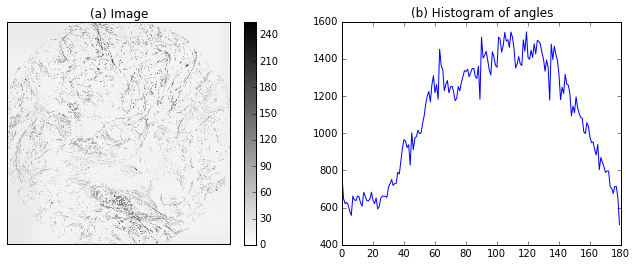
\includegraphics[width=0.8\textwidth]{hist_sum_anisotropic}
\caption{(a) Image which seems to be anisotropic to human eye. (b) Histogram of angles calculated by summing up the angle of top intensity pixels in Fourier spectrum. Histogram have a high count of angles from $\approx$ 40 to 160 degrees, making a broad peak.}
\label{fig:hist_sum_anisotropic}
\end{figure} % Results

\chapter{Discussion}

\section{Scan settings}
Selecting acceptable settings is a compromise between resolution, signal, noise and time. As water evaporates rather quick (maximum evaporation time was found to be an hour), scanning a whole slide in one job is not possible with any of the water objectives. This leaves us left with the 20x dry and 63x oil objective. As seen in table \ref{tab:obj_time} using 63x oil objective a scan job will take about twice as long as with a 20x dry objective. This was found to be an acceptable trade off between time and resolution, with a whole scan taking minimum two hours.

As we can see in figure \ref{fig:obj_comparison}, we have weaker signal with the 63x water objective compared to 20x dry. Although the gain of the detector is 50 Volt higher in image (a), this should not give difference of such magnitude. As a lot of things will effect the intensity, ranging all the way from laser power to mirror oscillation frequency, one should confirm the intensity range by taking a small test scan before scanning a whole slide.

One factor that is limiting to laser power, is HyD detector shutting down due getting several photons at the same time. A good solution to this problem has not been found. Limiting laser power will decrease amount of bright spots which is able to shut down HyD detector, but the problem is not completely excluded until setting laser power too low to generate any significant signal. It is suggested that one concentrate on forward PMT detectors until one can eliminate bright spots.

\section{Automation of the process}
Tile scan give limited options to adjusting a scan and also makes it hard to separate samples. Using matrix scan is therefor more appropriate for scanning slides where samples are spread over a large area. Also, a feature in the software called \textit{computer assisted microscopy} may be used for automatic adjusting of placement to wells.



\section{Quantification}

\subsection{Gradient}
Using gradient for quantifying fiber direction does not seem to be a good match. This is illustrated in figure \ref{fig:grad} and \ref{fig:grad_arr}, where a lot of random directions get generated. Especially angles which are multiples of 45 degrees get a high response, which is due to the nature of the data (being a two dimensional image). As one might imagine, a single pixel of high intensity (as noise often is), would generate gradients with magnitude of n$\cdot$45 degrees in the pixels around. This is not easily remedied with filtering, as one would simply create a "mountain" where the strong pixel is (and get the same effect further away from the pixel).

\begin{figure}[h]
\centering
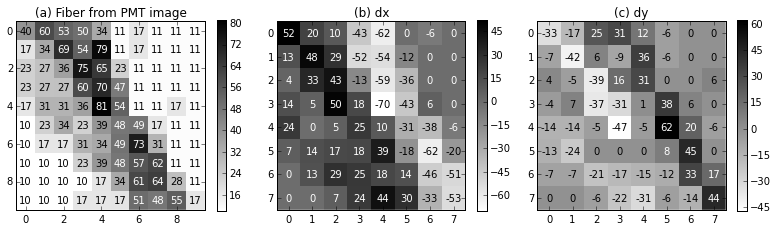
\includegraphics[width=\textwidth]{gradient}
\caption{(a) Section of image with strong signal from a fiber. Numbers in cells are intensity values of image. (b) X-component of gradient. (c) Y-component of gradient.}
\label{fig:grad}
\end{figure}

\begin{figure}[H]
\centering
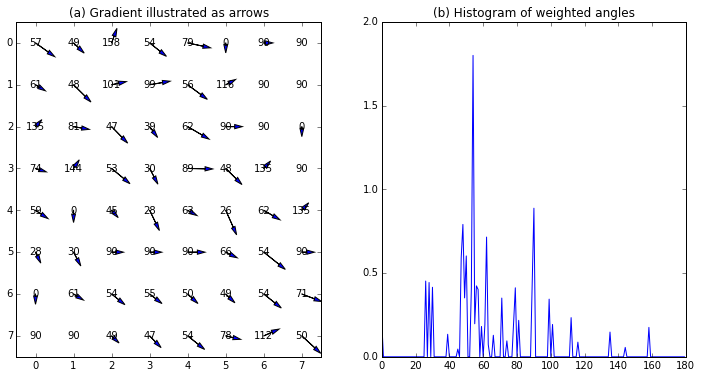
\includegraphics[width=\textwidth]{gradient_arrow}
\caption{(a) Gradient to image in figure \ref{fig:grad} (a) drawn as arrows. An angle of 90 degrees have been added to gradient to align the gradient in the same direction as the fiber. (b) The weighed histogram of angles to gradients in (a).}
\label{fig:grad_arr}
\end{figure}

A possible improvement could be to discard all but the strongest or averaged direction to gradients of sub images. Also, one could try to preprocess the image with some kind of edge detection and then using similar technique on a binary image.


\subsection{Frequency domain}
Line fitting of sub images in the Fourier image give good indication of strong fiber orientations. Lines with low correlation coefficient, as in figure \ref{fig:line_bad}, should be discarded to not include angles which are merely selected at random. A possibility to improve this technique is summing up angles instead of using line fit.

\begin{figure}[h]
\centering
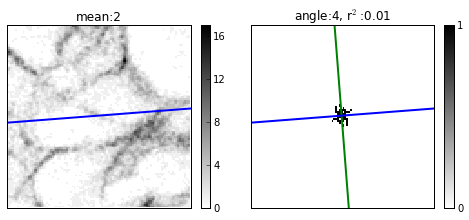
\includegraphics[width=0.66\textwidth]{ft_line_bad}
\caption{(a) Sub image of a sample. (b) Fourier spectrum and line fit. Note the low correlation coefficient r$^2$ = 0.01.}
\label{fig:line_bad}
\end{figure}

Summing up angles of highest intensities in Fourier spectrum seem to be good approach in detecting direction of fibers in image. In the images selected, the broadness of the peak in the histogram is a good measure of fiber direction anisotropy. This should be verified on a larger data set. One problem might be directions with similar angles, which may overlap in the histogram and broadening the peak. A possible solution to this is dividing the image into sub images as the previous Fourier algorithm. % Discussion

\chapter{Conclusion}
High quality images of collagen fiber has been collected in a structured fashion which may be used for further collection of data. Techniques for analysing the fiber orientation have been tested out. For further work, it is suggested that one should improve collection of images by using Computer Assisted Scanning, to make the collection more time efficient. For analysis it is suggested that one do machine learning on a large data set and try to predict outcome of patients. % Conclusion

\addtocontents{toc}{\vspace{2em}} % Add a gap in the Contents, for aesthetics

\addtocontents{toc}{\vspace{2em}}  % Add a gap in the Contents, for aesthetics
\backmatter

%% ----------------------------------------------------------------
\label{Bibliography}
\lhead{\emph{Bibliography}}  % Change the left side page header to "Bibliography"
\bibliographystyle{unsrtnat}  % Use the "unsrtnat" BibTeX style for formatting the Bibliography
\bibliography{Bibliography}  % The references (bibliography) information are stored in the file named "Bibliography.bib"

\end{document}  % The End
%% ----------------------------------------------------------------